% ============================================================
% Chương 6. Hiện thực  (chuẩn 2.1, 3.1, 3.2)
% Nguồn: docs/report_tv1.md mục 1.3, 1.4, 3; README.md; docs/tv3_marts.md; docs/contract.md
% ============================================================
\section{Hiện thực}
\label{sec:hien-thuc}

Chương này trình bày cách hiện thực từng thành phần của kiến trúc ở
chương~\ref{sec:kien-truc}: môi trường triển khai, quá trình ETL, việc nạp kho, điều phối,
các truy vấn nghiệp vụ và dashboard.

% ------------------------------------------------------------
\subsection{Môi trường triển khai}
\label{sec:moi-truong}

Toàn bộ hệ thống chạy trong các container được định nghĩa bằng Docker Compose. Container
ứng dụng chứa Python, Java, Spark và các thư viện, dùng chung cho ETL, kiểm thử và dashboard;
container PostgreSQL chứa kho đối chứng. Kafka và Airflow được tách thành các nhóm dịch vụ
(profile) riêng, chỉ khởi động khi cần, để máy cá nhân không phải chạy những thành phần không
dùng tới. Khóa truy cập Google Cloud và các biến cấu hình được đặt ngoài kho mã nguồn.

Mỗi bước của pipeline là một lệnh trong Makefile, và một lệnh tổng hợp chạy toàn bộ các bước
theo thứ tự, dừng ngay ở bước lỗi đầu tiên và ghi lại thời gian từng bước. Trên máy chưa có
khóa Google Cloud, một biến thể của lệnh này bỏ qua bước nạp BigQuery, nên mọi thành viên
đều dựng được kho đầy đủ trên Parquet và PostgreSQL.

Phiên bản của toàn bộ 70 gói Python, kể cả các gói phụ thuộc gián tiếp, được khóa cố định
trong một file khóa (lock file). Biện pháp này được bổ sung sau khi một lần dựng lại image tự
động cài các phiên bản mới của DuckDB, pandas và pytest, làm hỏng một số lệnh gọi DuckDB và
bài kiểm thử. Từ đó, image dựng lại ở bất kỳ máy nào đều cài đúng cùng một bộ thư viện.

% ------------------------------------------------------------
\subsection{ETL bằng Spark}
\label{sec:etl}

\subsubsection{Các bước và thời gian}

Quá trình ETL gồm bốn bước Spark, tiếp theo là hai bước nạp và một bước kiểm thử
(Bảng~\ref{tab:etl-thoi-gian}). Thời gian được đo trên máy 16 CPU, cấp 8 GB RAM cho
container và 3 GB cho Spark driver; toàn bộ pipeline dựng lại kho từ đầu trong khoảng 5 phút.

\begin{table}[htbp]
\centering
\small
\begin{tabular}{|l|l|r|}
\hline
\textbf{Bước} & \textbf{Nội dung} & \textbf{Thời gian (s)} \\ \hline
Staging & 7 file CSV $\rightarrow$ 7 bảng Parquet & 46,0 \\ \hline
Dimension & Làm sạch, dựng 5 dimension và \texttt{fact\_enrollment} & 38,4 \\ \hline
Fact & Dựng \texttt{fact\_vle\_daily} và \texttt{fact\_submission} & 31,6 \\ \hline
Bảng tiến độ theo tuần & Dựng \texttt{fact\_student\_week} & 33,2 \\ \hline
Nạp BigQuery & 9 bảng & 83,5 \\ \hline
Nạp PostgreSQL & 9 bảng & 25,1 \\ \hline
Kiểm thử & Toàn bộ bộ kiểm thử & 45,1 \\ \hline
\textbf{Tổng} & & \textbf{303,0} \\ \hline
\end{tabular}
\caption{Thời gian các bước khi dựng lại toàn bộ kho}
\label{tab:etl-thoi-gian}
\end{table}

Bảng nặng nhất là bảng click: 10.655.280 dòng đầu vào được gộp còn 8.459.320 dòng. Riêng
việc ghi bảng này ra Parquet mất 17,4 giây và nạp lên BigQuery mất 30,0 giây.

\subsubsection{Nguyên tắc làm sạch}

Quá trình làm sạch tuân theo bốn nguyên tắc. Thứ nhất, không xóa dòng và không sửa giá trị
gốc; mọi vấn đề chất lượng được biểu diễn bằng cột cờ kiểu \texttt{BOOL}
(mục~\ref{sec:luan-ly}), để người phân tích tự quyết định lọc hay giữ. Thứ hai, ngày được giữ
ở dạng số nguyên tương đối so với ngày khai giảng như trong dữ liệu nguồn. Thứ ba, số tuần
được tính bằng phép làm tròn xuống \texttt{FLOOR(date / 7)}: phép chia nguyên của DuckDB và
BigQuery làm tròn về 0, khiến ngày $-1$ rơi vào tuần 0 thay vì tuần $-1$, nên công thức này
được chốt chung cho ETL và mọi truy vấn, kèm một bài kiểm thử riêng. Thứ tư, số dòng của mỗi
bảng được kiểm tra ngay sau khi ghi và so với con số đã chốt trong hợp đồng dữ liệu của nhóm.

\subsubsection{Xử lý các vấn đề của dữ liệu nguồn}

Bảng~\ref{tab:xu-ly} trình bày cách xử lý các vấn đề đã nêu ở mục~\ref{sec:van-de-du-lieu}.

\begin{table}[htbp]
\centering
\footnotesize
\begin{tabularx}{\textwidth}{|p{4.0cm}|X|r|}
\hline
\textbf{Vấn đề} & \textbf{Cách xử lý} & \textbf{Số dòng} \\ \hline
Bảng click có nhiều dòng trùng khóa & Gộp thành một dòng mỗi khóa, cộng số click, ghi số dòng gốc vào cột \texttt{n\_records}; tổng click giữ nguyên 39.605.099 & 10.655.280 $\rightarrow$ 8.459.320 \\ \hline
Thiếu nhóm IMD & Ghi \texttt{'Unknown'}, gắn cờ \texttt{imd\_unknown} & 971 sinh viên \\ \hline
Nhóm IMD ghi \texttt{10-20} thay vì \texttt{10-20\%} & Thống nhất thành \texttt{10-20\%}, tránh tách một nhóm thành hai khi tổng hợp (BR6) & \\ \hline
Bài thi cuối kỳ thiếu hạn nộp & Gán hạn nộp bằng độ dài đợt, giữ cột gốc, gắn cờ \texttt{deadline\_imputed} & 11 bài \\ \hline
Nhóm tuổi thay đổi giữa các lần đăng ký & Đặt nhóm tuổi ở \texttt{fact\_enrollment} thay vì \texttt{dim\_student} & 72 sinh viên \\ \hline
Thiếu ngày đăng ký & Giữ \texttt{NULL}, gắn cờ \texttt{reg\_date\_missing} & 45 lượt \\ \hline
Kết quả cuối kỳ không khớp với ngày rút & Giữ nguyên, gắn cờ \texttt{result\_inconsistent} & 102 lượt \\ \hline
Bài đã nộp nhưng không có điểm & Giữ \texttt{NULL}, gắn cờ \texttt{score\_missing} & 173 bài \\ \hline
Bài chuyển điểm từ đợt trước & Không tính trễ hạn; số ngày trễ để \texttt{NULL} & 1.909 bài \\ \hline
Ngày ghi của CMA không phải hạn nộp thật & Cờ \texttt{is\_late} chỉ xét TMA; nếu xét cả CMA thì 49.323 bài bị tính trễ sai & 16.320 bài trễ \\ \hline
\end{tabularx}
\caption{Cách xử lý các vấn đề của dữ liệu nguồn}
\label{tab:xu-ly}
\end{table}

\subsubsection{Bảng tiến độ theo tuần và chống rò rỉ nhãn}

Bảng \texttt{fact\_student\_week} là ảnh chụp tiến độ của mỗi lượt đăng ký theo tuần, phục
vụ cảnh báo sớm (BR4) và theo dõi tiến độ (BR7). Mỗi lượt đăng ký có đủ các tuần từ tuần $-4$
đến tuần cuối của đợt, kể cả những tuần không có click (ghi giá trị 0) và những tuần sau khi
sinh viên đã rút; cột \texttt{is\_enrolled} cho biết sinh viên còn học tại tuần đó hay không.
Các cột lũy kế, như tổng click, số bài đã nộp và điểm trung bình, tuân theo quy tắc as-of
(mục~\ref{sec:luan-ly}).

Bảng này không chứa kết quả cuối kỳ. Kết quả cuối kỳ chỉ nằm ở \texttt{fact\_enrollment} và
chỉ được nối vào khi đánh giá độ chính xác của danh sách cảnh báo sau khi đợt học kết thúc.
Thiết kế này được kiểm chứng bằng hai bài kiểm thử: một bài bảo đảm bảng không có cột nhãn,
một bài đảo ngược toàn bộ kết quả cuối kỳ rồi lập lại danh sách cảnh báo tuần 4 và xác nhận
danh sách không thay đổi.

% ------------------------------------------------------------
\subsection{Nạp kho}
\label{sec:nap-kho}

Trên BigQuery, mỗi bảng được nạp bằng một load job ở chế độ thay thế toàn bộ bảng
(\texttt{WRITE\_TRUNCATE}). Load job thành công thì bảng mới thay bảng cũ trong một lần; thất
bại thì bảng cũ được giữ nguyên, nên không bao giờ có trạng thái nạp dở dang. Sau khi nạp,
số dòng của bảng trên BigQuery được so với số dòng trên Parquet.

Trên PostgreSQL, mỗi bảng được nạp trong một giao dịch: xóa bảng cũ, tạo bảng, nạp dữ liệu
bằng lệnh \texttt{COPY}, thêm khóa chính, rồi mới xác nhận giao dịch; sau đó cập nhật thống kê
cho bộ tối ưu truy vấn. Số dòng của cả 9 bảng trên PostgreSQL được so với Parquet và BigQuery.

Mọi bước của pipeline đều ghi đè thay vì ghi thêm: Spark ghi Parquet ở chế độ overwrite,
BigQuery thay thế toàn bộ bảng, PostgreSQL tạo lại bảng trong cùng giao dịch. Nhờ vậy, chạy
lại pipeline bao nhiêu lần cũng cho cùng một kết quả mà không sinh dòng trùng (idempotent);
tính chất này có bài kiểm thử nạp hai lần liên tiếp.

Ngoài kho chính, một bản mở rộng quy mô gấp 5 lần được dựng để đo hiệu năng. Mỗi sinh viên
được nhân thành 5 bản với mã sinh viên khác nhau, kéo theo toàn bộ dữ liệu fact của sinh viên
đó; các dimension tĩnh được giữ nguyên. Vì nhân bản nguyên vẹn, mọi tỷ lệ của bản mở rộng
bằng kho gốc, chỉ khối lượng tăng 5 lần: bảng click đạt 42,3 triệu dòng, khoảng 2,6 GB trên
BigQuery.

% ------------------------------------------------------------
\subsection{Xử lý stream}
\label{sec:stream}

Nhánh stream tính lại tổng click theo sinh viên, đợt học và tuần bằng Spark Structured
Streaming, rồi đối chiếu với bảng tiến độ theo tuần của batch. Có hai nguồn cho cùng một phép
tính: một thư mục nhận file theo từng ngày (không cần thêm hệ thống nào), và Kafka (gần với hệ
thống thật hơn, có watermark để giới hạn bộ nhớ). Bảng~\ref{tab:stream-buoc} tóm tắt các bước.

\begin{table}[htbp]
\centering
\small
\begin{tabularx}{\textwidth}{|p{2.2cm}|X|}
\hline
\textbf{Bước} & \textbf{Nội dung} \\ \hline
Chia ngày & Chia \texttt{studentVle} thành 295 file, mỗi file một ngày (ngày $-25$ đến 269) \\ \hline
Gửi & Nguồn thư mục: thả từng file theo thứ tự ngày; file được chép vào tên ẩn rồi đổi tên, nên Spark không đọc phải file đang chép dở. Nguồn Kafka: mỗi dòng click là một message lên topic \texttt{oulad.clicks} (4 partition), khóa là mã sinh viên nên click của một sinh viên luôn giữ đúng thứ tự \\ \hline
Xử lý & Spark gom click theo cửa sổ 7 ngày của thời gian sự kiện, ghi ở chế độ \texttt{update}: mỗi micro-batch chỉ ghi các dòng vừa thay đổi, kèm số thứ tự micro-batch \\ \hline
Phục vụ & Mỗi micro-batch được nạp lên BigQuery; trang dashboard đọc giá trị mới nhất của mỗi dòng \\ \hline
Đối chiếu & Lấy giá trị mới nhất của mỗi dòng, cộng dồn ra \texttt{clicks\_cum}, so với bảng tiến độ theo tuần của batch \\ \hline
\end{tabularx}
\caption{Các bước của nhánh stream}
\label{tab:stream-buoc}
\end{table}

\textbf{Thời gian sự kiện và watermark.} OULAD chỉ có số ngày tính từ khai giảng, không có ngày
giờ thật. Mỗi click được gán mốc thời gian là ngày 06/01/2000 cộng số ngày đó; ngày gốc này cách
01/01/1970 đúng 1.566 tuần, mà cửa sổ 7 ngày của Spark được tính từ 01/01/1970, nên mỗi cửa sổ
trùng đúng một tuần của OULAD. Watermark là mốc thời gian sự kiện lớn nhất đã thấy trừ đi 7 ngày;
khi watermark vượt qua cuối một tuần, Spark coi tuần đó đã đóng và xóa nó khỏi bộ nhớ, click nào
của tuần đó đến sau sẽ bị bỏ và được đếm lại. Chế độ \texttt{update} được chọn thay cho
\texttt{append} vì \texttt{append} chỉ ghi một tuần khi tuần đó đã đóng, nên một hai tuần cuối sẽ
không bao giờ được ghi.

\textbf{Không trùng, không mất.} Producer bật chế độ idempotent nên gửi lại khi lỗi mạng không
tạo message trùng; Spark lưu offset đã đọc vào checkpoint nên khởi động lại thì đọc tiếp đúng chỗ;
mỗi micro-batch ghi đè vào thư mục riêng của nó nên chạy lại một micro-batch không sinh dòng trùng.
Trên BigQuery, gói Sandbox không cho dùng lệnh sửa dữ liệu, nên mỗi micro-batch được ghi thêm vào
một bảng nhật ký, và một view chọn dòng có số thứ tự micro-batch lớn nhất cho mỗi khóa; micro-batch
có bị nạp hai lần thì view vẫn trả đúng một dòng.

\begin{table}[htbp]
\centering
\small
\begin{tabular}{|l|r|r|}
\hline
\textbf{Chỉ số} & \textbf{Nguồn thư mục} & \textbf{Nguồn Kafka} \\ \hline
Số dòng click đưa vào & 10.655.280 & 10.655.280 \\ \hline
Số micro-batch & 44 & 63 \\ \hline
Thời gian & 97,5 s & 130,3 s \\ \hline
Trạng thái lúc lớn nhất & 627.031 khóa & 65.274 khóa \\ \hline
Trạng thái lúc kết thúc & 627.031 khóa & 4.803 khóa \\ \hline
Dòng bị watermark bỏ & không có watermark & 0 \\ \hline
Lệch so với batch (1.342.949 dòng) & 0 & 0 \\ \hline
Tổng click & 39.605.099 & 39.605.099 \\ \hline
\end{tabular}
\caption{Kết quả hai nguồn stream so với batch (lần chạy ngày 31/10/2026)}
\label{tab:stream-ket-qua}
\end{table}

Bảng~\ref{tab:stream-ket-qua} cho thấy hai nguồn ra cùng kết quả và khớp batch từng dòng.
Khác biệt chính nằm ở bộ nhớ: không có watermark, Spark giữ tổng click của mọi tuần đã gặp tới
cuối lần chạy, nên với luồng chạy mãi bộ nhớ sẽ tăng không giới hạn; có watermark, trạng thái lúc
lớn nhất nhỏ hơn khoảng 10 lần và được dọn gần hết khi luồng kết thúc. Cái giá của watermark là
dữ liệu đến quá trễ bị bỏ: khi cố ý giữ lại 0,1\% số click và gửi sau cùng, Spark bỏ đúng các
click đó và kết quả lệch so với batch. Bản Kafka chậm hơn 33 giây, chủ yếu do gửi 10,6 triệu
message qua mạng và phân tích JSON.

Khi bật ghi lên BigQuery, mỗi micro-batch là một load job mất khoảng 5 giây dù chỉ vài chục
nghìn dòng. Spark đợi job xong mới chạy micro-batch sau, nên click dồn lại và micro-batch lớn hơn
(44 thay vì 63); dữ liệu không mất, nhưng độ trễ từ lúc click vào Kafka tới lúc hiện trên
dashboard khoảng 5--10 giây. Muốn nhanh hơn cần ghi stream trực tiếp vào BigQuery, vốn phải bật
tính phí.

% ------------------------------------------------------------
\subsection{Điều phối bằng Airflow}
\label{sec:airflow}

Lệnh tổng hợp ở mục~\ref{sec:moi-truong} chạy tuần tự, cần người khởi động và dừng hẳn khi
gặp lỗi. Một DAG Airflow chạy cùng các bước đó nhưng bổ sung các cơ chế điều phối. Thứ tự
các task như sau, trong đó hai bước nạp chạy song song:

\begin{center}
\small
\texttt{wait\_raw\_csv} $\rightarrow$ \texttt{staging} $\rightarrow$ \texttt{dims}
$\rightarrow$ \texttt{facts} $\rightarrow$ \texttt{student\_week}
$\rightarrow$ \texttt{quality\_gate} \\
$\rightarrow$ (\texttt{load\_bq} $\parallel$ \texttt{load\_pg})
$\rightarrow$ \texttt{test\_all} $\rightarrow$ \texttt{give\_back\_files}
\end{center}

\begin{table}[htbp]
\centering
\small
\begin{tabularx}{\textwidth}{|p{2.8cm}|X|X|}
\hline
\textbf{Cơ chế} & \textbf{Cách hiện thực} & \textbf{Lý do} \\ \hline
Lập lịch & Chạy lúc 2 giờ sáng (UTC) hằng ngày; không chạy bù các ngày đã qua; tối đa một lần chạy cùng lúc & Hai lần chạy đồng thời sẽ ghi đè dữ liệu của nhau \\ \hline
Chờ dữ liệu đầu vào & Sensor kiểm tra đủ 7 file CSV mỗi phút, tối đa 1 giờ, không chiếm chỗ chạy trong lúc chờ & Nguồn đến muộn thì chờ thay vì báo lỗi ngay \\ \hline
Cổng chất lượng & Chạy các bài kiểm thử trên kho Parquet trước khi nạp & Lỗi thì dừng; BigQuery và PostgreSQL giữ bản cũ \\ \hline
Chạy song song & Nạp BigQuery và nạp PostgreSQL cùng lúc & Hai bước chỉ đọc Parquet, không phụ thuộc nhau \\ \hline
Chạy lại khi lỗi & Mỗi task thử lại một lần sau 2 phút; quá 20 phút thì dừng & An toàn vì mọi bước đều ghi đè \\ \hline
Báo lỗi & Task lỗi hẳn thì ghi một bản ghi vào file log và gửi webhook (Discord, Slack) nếu được cấu hình & Lịch chạy lúc 2 giờ sáng, không có người theo dõi trực tiếp \\ \hline
\end{tabularx}
\caption{Các cơ chế điều phối của DAG}
\label{tab:co-che-airflow}
\end{table}

Mỗi task chỉ gọi đúng một lệnh trong Makefile, nên logic ETL không phụ thuộc vào Airflow và
pipeline vẫn chạy được bằng tay khi không khởi động Airflow. Airflow chạy trên chính image của
ứng dụng nhưng trong một môi trường Python riêng, để các task gọi được Spark như khi chạy tay
mà thư viện của Airflow không ghi đè phiên bản thư viện của hệ thống. Lịch sử chạy được lưu
trong PostgreSQL, cho phép dùng \texttt{LocalExecutor} để chạy các task song song.

\begin{table}[htbp]
\centering
\small
\begin{tabular}{|l|r|}
\hline
\textbf{Task} & \textbf{Thời gian (s)} \\ \hline
\texttt{wait\_raw\_csv} & 0,1 \\ \hline
\texttt{staging} & 21,7 \\ \hline
\texttt{dims} & 17,2 \\ \hline
\texttt{facts} & 20,6 \\ \hline
\texttt{student\_week} & 33,5 \\ \hline
\texttt{quality\_gate} (110 bài kiểm thử) & 3,1 \\ \hline
\texttt{load\_bq} $\parallel$ \texttt{load\_pg} & 76,3 $\parallel$ 22,9 \\ \hline
\texttt{test\_all} & 43,8 \\ \hline
\texttt{give\_back\_files} & 0,8 \\ \hline
\textbf{Cả lần chạy} & \textbf{222,8} \\ \hline
\end{tabular}
\caption{Thời gian một lần chạy DAG theo lịch}
\label{tab:airflow-thoi-gian}
\end{table}

Nếu chạy tuần tự, tổng thời gian các task là 240 giây; chạy song song hai bước nạp tiết kiệm
đúng thời gian của bước ngắn hơn, khoảng 23 giây. Thời gian Airflow chờ giữa hai task cộng lại
khoảng 4,5 giây cho cả lần chạy, không đáng kể so với các bước Spark. Cổng chất lượng chỉ tốn
3 giây nhưng ngăn được việc đẩy dữ liệu sai lên kho mà dashboard đang đọc.

% ------------------------------------------------------------
\subsection{Truy vấn nghiệp vụ và bảng tổng hợp sẵn}
\label{sec:truy-van}

SQL của 20 câu hỏi mẫu được viết theo cú pháp chung, không dùng hàm riêng của hệ quản trị
nào; trung vị và phân vị được tính bằng đánh số dòng và nội suy tuyến tính thay vì các hàm
phân vị đặc thù. Nhờ vậy, cùng một file SQL chạy được trên BigQuery, PostgreSQL và DuckDB, và
kết quả trên ba hệ có thể đối chiếu trực tiếp với nhau.

Hai bảng tổng hợp sẵn (data mart) được dựng trên BigQuery cho hai trang có truy vấn nặng nhất
(Bảng~\ref{tab:mart}). Cả hai được tạo bằng câu lệnh \texttt{CREATE OR REPLACE TABLE ... AS
SELECT} chạy trực tiếp trên các bảng của kho, nên thay thế toàn bộ nội dung mỗi lần làm mới.
Việc làm mới hiện được thực hiện thủ công, chưa nằm trong DAG.

\begin{table}[htbp]
\centering
\small
\begin{tabularx}{\textwidth}{|p{3.6cm}|p{3.4cm}|X|}
\hline
\textbf{Data mart} & \textbf{Grain} & \textbf{Nội dung} \\ \hline
\texttt{tv3\_br2\_weekly\_mart} & đợt $\times$ tuần $\times$ loại học liệu & Số sinh viên còn học, tổng click, click trung bình mỗi sinh viên, tỷ trọng từng loại học liệu (BR2) \\ \hline
\texttt{tv3\_br3\_student\_mart} & đợt $\times$ sinh viên & Click trước hạn bài TMA đầu tiên, điểm bài đó, cỡ mẫu và hệ số Spearman của đợt (BR3) \\ \hline
\end{tabularx}
\caption{Hai bảng tổng hợp sẵn trên BigQuery}
\label{tab:mart}
\end{table}

% ------------------------------------------------------------
\subsection{Dashboard}
\label{sec:dashboard}

Dashboard được xây dựng bằng Streamlit, gồm 9 trang chia theo nhóm người dùng
(Bảng~\ref{tab:trang}). Mỗi nhóm chỉ thấy các trang phục vụ nhu cầu của mình, và một số trang
dùng chung lựa chọn đợt học để người dùng không phải chọn lại khi chuyển trang.

\begin{table}[htbp]
\centering
\small
\begin{tabularx}{\textwidth}{|l|X|l|}
\hline
\textbf{Nhóm} & \textbf{Trang} & \textbf{Yêu cầu} \\ \hline
Chung & Tổng quan & \\ \hline
Giảng viên & Hoạt động học tập; Nộp bài và điểm & BR1, BR2, BR3 \\ \hline
Cố vấn học tập & Cảnh báo sớm và rút lui & BR4, BR5 \\ \hline
Lãnh đạo khoa & Khoảng cách IMD & BR6 \\ \hline
Sinh viên & Tiến độ so với lớp; Diễn đàn tuần 5 & BR7, BR8 \\ \hline
Hệ thống & Chất lượng và benchmark; Click thời gian thực & \\ \hline
\end{tabularx}
\caption{Các trang của dashboard theo nhóm người dùng}
\label{tab:trang}
\end{table}

% TODO: mỗi nhóm người dùng một ảnh chụp màn hình, ví dụ:
% \begin{figure}[htbp]
% \centering
% 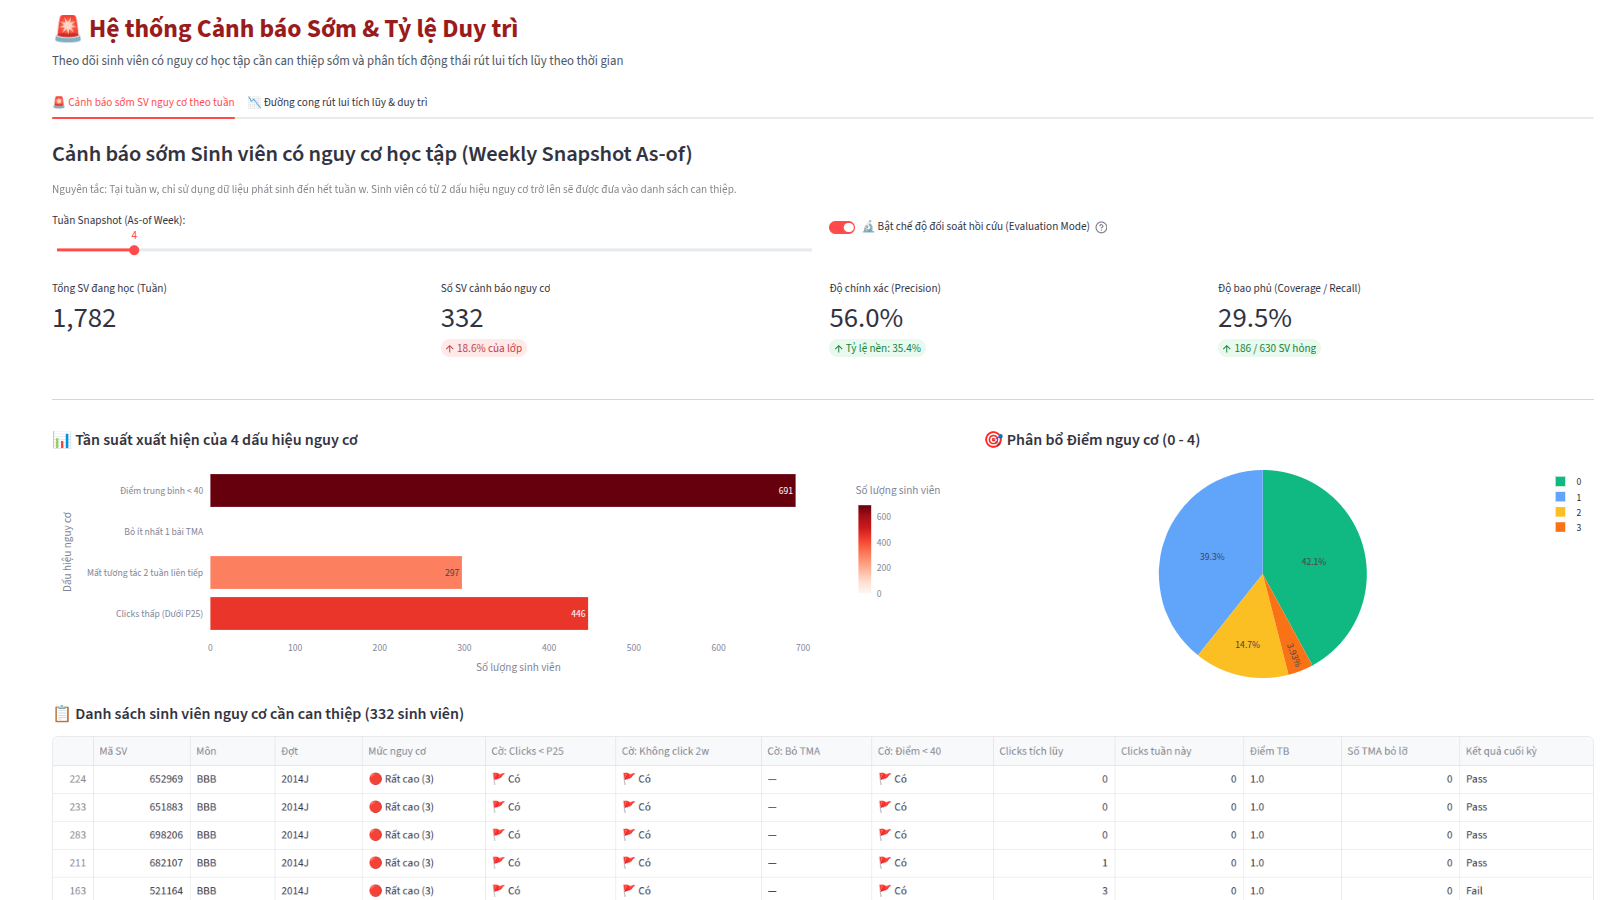
\includegraphics[width=\textwidth]{Images/dashboard_canh_bao.png}
% \caption{Trang Cảnh báo sớm: danh sách sinh viên có nguy cơ tại tuần 4}
% \label{fig:dashboard-canh-bao}
% \end{figure}
